% ******************************* PhD Thesis Template **************************
% Please have a look at the README.md file for info on how to use the template

\documentclass[a4paper,11pt, oneside, times, numbered, custommargin]{Classes/PhDThesisPSnPDF}
% chapter, print, oneside, draftclassic

% ******************************************************************************
% ******************************* Class Options ********************************
% *********************** See README for more details **************************
% ******************************************************************************

% `a4paper'(The University of Cambridge PhD thesis guidelines recommends a page
% size a4 - default option) or `a5paper': A5 Paper size is also allowed as per
% the Cambridge University Engineering Deparment guidelines for PhD thesis
%
% `11pt' or `12pt'(default): Font Size 10pt is NOT recommended by the University
% guidelines
%
% `oneside' or `twoside'(default): Printing double side (twoside) or single
% side.
%
% `print': Use `print' for print version with appropriate margins and page
% layout. Leaving the options field blank will activate Online version.
%
% `index': For index at the end of the thesis
%
% `draftclassic': For draft mode without loading any images (same as draft in book)
%
% `draft': Special draft mode with line numbers, images, and water mark with
% timestamp and custom text. Position of the text can also be modified.
%
% `abstract': To generate only the title page and abstract page with
% dissertation title and name, to submit to the Student Registry
%
% `chapter`: This option enables only the specified chapter and it's references
%  Useful for review and corrections.
%
% ************************* Custom Page Margins ********************************
%
% `custommargin`: Use `custommargin' in options to activate custom page margins,
% which can be defined in the preamble.tex. Custom margin will override
% print/online margin setup.
%
% *********************** Choosing the Fonts in Class Options ******************
%
% `times' : Times font with math support. (The Cambridge University guidelines
% recommend using times)
%
% `fourier': Utopia Font with Fourier Math font (Font has to be installed)
%            It's a free font.
%
% `customfont': Use `customfont' option in the document class and load the
% package in the preamble.tex
%
% default or leave empty: `Latin Modern' font will be loaded.
%
% ********************** Choosing the Bibliography style ***********************
%
% `authoryear': For author-year citation eg., Krishna (2013)
%
% `numbered': (Default Option) For numbered and sorted citation e.g., [1,5,2]
%
% `custombib': Define your own bibliography style in the `preamble.tex' file.
%              `\RequirePackage[square, sort, numbers, authoryear]{natbib}'.
%              This can be also used to load biblatex instead of natbib
%              (See Preamble)
%
% **************************** Choosing the Page Style *************************
%
% `default (leave empty)': For Page Numbers in Header (Left Even, Right Odd) and
% Chapter Name in Header (Right Even) and Section Name (Left Odd). Blank Footer.
%
% `PageStyleI': Chapter Name next & Page Number on Even Side (Left Even).
% Section Name & Page Number in Header on Odd Side (Right Odd). Footer is empty.
%
% `PageStyleII': Chapter Name on Even Side (Left Even) in Header. Section Number
% and Section Name in Header on Odd Side (Right Odd). Page numbering in footer

% Uncomment to change page style
%\pagestyle{PageStyleII}



% **************************** Custumize chapter display *************************

\usepackage{titlesec}
\titleformat{\chapter}[hang]{\normalfont\bfseries\huge}{\thechapter}{0.5em}{}
%\titleformat{hcommandi}[hshapei]{hformati}{hlabeli}{hsepi}{hbefore-codei}[hafter-codei]
%\sffamily\itshape

% ********************************** Preamble **********************************
% Preamble: Contains packages and user-defined commands and settings
% ******************************************************************************
% ****************************** Custom Margin *********************************

% Add `custommargin' in the document class options to use this section
% Set {innerside margin / outerside margin / topmargin / bottom margin}  and
% other page dimensions
\ifsetCustomMargin
  \RequirePackage[left=30mm,right=30mm,top=35mm,bottom=30mm]{geometry}
  \setFancyHdr % To apply fancy header after geometry package is loaded
\fi

% Add spaces between paragraphs
%\setlength{\parskip}{0.5em}

\setlength{\parindent}{0pt}

% Ragged bottom avoids extra whitespaces between paragraphs
\raggedbottom
% To remove the excess top spacing for enumeration, list and description
%\usepackage{enumitem}
%\setlist[enumerate,itemize,description]{topsep=0em}

% *****************************************************************************
% ******************* Fonts (like different typewriter fonts etc.)*************

% Add `customfont' in the document class option to use this section

\ifsetCustomFont
  % Set your custom font here and use `customfont' in options. Leave empty to
  % load computer modern font (default LaTeX font).
  %\RequirePackage{helvet}

  % For use with XeLaTeX
  %  \setmainfont[
  %    Path              = ./libertine/opentype/,
  %    Extension         = .otf,
  %    UprightFont = LinLibertine_R,
  %    BoldFont = LinLibertine_RZ, % Linux Libertine O Regular Semibold
  %    ItalicFont = LinLibertine_RI,
  %    BoldItalicFont = LinLibertine_RZI, % Linux Libertine O Regular Semibold Italic
  %  ]
  %  {libertine}
  %  % load font from system font
  %  \newfontfamily\libertinesystemfont{Linux Libertine O}
\fi

% *****************************************************************************
% **************************** Custom Packages ********************************
\usepackage{titlesec}
\usepackage{xcolor}
\usepackage{ulem}
\usepackage{enumitem}




% ************************* Algorithms and Pseudocode **************************

%\usepackage{algpseudocode}


% ********************Captions and Hyperreferencing / URL **********************

% Captions: This makes captions of figures use a boldfaced small font.
%\RequirePackage[small,bf]{caption}

\RequirePackage[font=small]{caption}
\renewcommand{\figurename}{Fig.} %to support older versions of captions.sty
\DeclareCaptionFont{red}{\color{red}}
\DeclareCaptionFont{green}{\color{green}}
\DeclareCaptionFont{blue}{\color{blue}}
\DeclareCaptionFont{gray}{\color{gray}}
\captionsetup{labelfont={gray,bf},textfont=gray}



% *************************** Graphics and figures *****************************

%\usepackage{rotating}
%\usepackage{wrapfig}

% Uncomment the following two lines to force Latex to place the figure.
% Use [H] when including graphics. Note 'H' instead of 'h'
%\usepackage{float}
%\restylefloat{figure}

% Subcaption package is also available in the sty folder you can use that by
% uncommenting the following line
% This is for people stuck with older versions of texlive
%\usepackage{sty/caption/subcaption}
\usepackage{subcaption}

% ********************************** Tables ************************************
\usepackage{booktabs} % For professional looking tables
\usepackage{multirow}

%\usepackage{multicol}
%\usepackage{longtable}
%\usepackage{tabularx}


% *********************************** SI Units *********************************
\usepackage{siunitx} % use this package module for SI units


% ******************************* Line Spacing *********************************

% Choose linespacing as appropriate. Default is one-half line spacing as per the
% University guidelines

% \doublespacing
% \onehalfspacing
\singlespacing


% ************************ Formatting / Footnote *******************************

% Don't break enumeration (etc.) across pages in an ugly manner (default 10000)
%\clubpenalty=500
%\widowpenalty=500

%\usepackage[perpage]{footmisc} %Range of footnote options


% *****************************************************************************
% *************************** Bibliography  and References ********************

%\usepackage{cleveref} %Referencing without need to explicitly state fig /table

% Add `custombib' in the document class option to use this section
\ifuseCustomBib
   \RequirePackage[square, sort, numbers, authoryear]{natbib} % CustomBib

% If you would like to use biblatex for your reference management, as opposed to the default `natbibpackage` pass the option `custombib` in the document class. Comment out the previous line to make sure you don't load the natbib package. Uncomment the following lines and specify the location of references.bib file

%\RequirePackage[backend=biber, style=numeric-comp, citestyle=numeric, sorting=nty, natbib=true]{biblatex}
%\bibliography{References/SDP.bib} %Location of references.bib only for biblatex

\fi

% changes the default name `Bibliography` -> `References'
\renewcommand{\bibname}{References}


% ******************************************************************************
% ************************* User Defined Commands ******************************
% ******************************************************************************

% *********** To change the name of Table of Contents / LOF and LOT ************

%\renewcommand{\contentsname}{My Table of Contents}
%\renewcommand{\listfigurename}{My List of Figures}
%\renewcommand{\listtablename}{My List of Tables}


% ********************** TOC depth and numbering depth *************************

\setcounter{secnumdepth}{2}
\setcounter{tocdepth}{2}


% ******************************* Nomenclature *********************************

% To change the name of the Nomenclature section, uncomment the following line

%\renewcommand{\nomname}{Symbols}


% ********************************* Appendix ***********************************

% The default value of both \appendixtocname and \appendixpagename is `Appendices'. These names can all be changed via:

%\renewcommand{\appendixtocname}{List of appendices}
%\renewcommand{\appendixname}{Appndx}

% *********************** Configure Draft Mode **********************************

% Uncomment to disable figures in `draft'
%\setkeys{Gin}{draft=true}  % set draft to false to enable figures in `draft'

% These options are active only during the draft mode
% Default text is "Draft"
%\SetDraftText{DRAFT}

% Default Watermark location is top. Location (top/bottom)
%\SetDraftWMPosition{bottom}

% Draft Version - default is v1.0
%\SetDraftVersion{v1.1}

% Draft Text grayscale value (should be between 0-black and 1-white)
% Default value is 0.75
%\SetDraftGrayScale{0.8}


% ******************************** Todo Notes **********************************
%% Uncomment the following lines to have todonotes.

\ifsetDraft
	\usepackage[colorinlistoftodos]{todonotes}
	\newcommand{\mynote}[1]{\todo[author=kks32,size=\small,inline,color=green!40]{#1}}
\else
	\newcommand{\mynote}[1]{}
	\newcommand{\listoftodos}{}
\fi

% Example todo: \mynote{Hey! I have a note}

% ************************ Thesis Information & Meta-data **********************
% Thesis title and author information, reference file for biblatex
% ************************ Thesis Information & Meta-data **********************

%% The title of the thesis
\title{Evaluate Prediction Accuracy of SOTA Branch Predictors on WSC traces}
%\texorpdfstring is used for PDF metadata. Usage:
%\texorpdfstring{LaTeX_Version}{PDF Version (non-latex)} eg.,
%\texorpdfstring{$sigma$}{sigma}

%% Subtitle (Optional)
%\subtitle{Using the CUED template}

\author{Derek Jinyu Dong (3035636987)}

%% Department (eg. Department of Engineering, Maths, Physics)
\dept{}

%% University and Crest
\university{}

% Crest minimum should be 30mm.
\HKUcrest{
\includegraphics[width=0.6\textwidth]{Figs/logo_CECD_C.png}}
\HUAWEIcrest{
\includegraphics[width=0.25\textwidth]{Figs/HUAWEI.png}}

%% Use this crest, if you are using the college crest
%% Crest long miminum should be 65mm
%\crest{
\includegraphics[width=0.45\textwidth]{University_Crest_Long}}

%% College shield [optional] 
% Crest minimum should be 30mm.
%\collegeshield{
\includegraphics[width=0.2\textwidth]{CollegeShields/Kings}}


%% Supervisor (optional)
%% for multiple supervisors, append each supervisor with the \newline command
\supervisor{Dr Artemiy Margaritov (HUAWEI)}

%% Supervisor Role (optional) - Supervisor (default) or advisor
%\supervisorrole{\textbf{Supervisor: }}
%% if no title is desired:
% \supervisorrole{}

%% Supervisor line width: required to align supervisors
\supervisorlinewidth{0.56\textwidth}

%% Advisor (optional)
%% for multiple advisors, append each advisor with the \newline command
\advisor{Prof Hayden K.H. So}
     
%% Advisor Role (optional) - Advisor (default) or leave empty
\advisorrole{Second Examiner: }
%% if no title is required
% \advisorrole{}

%% Advisor line width: required to align supervisors
\advisorlinewidth{0.34\textwidth}


%% You can redefine the submission text:
% Default as per the University guidelines:
% ``This dissertation is submitted for the degree of''
\renewcommand{\submissiontext}{ELEC4848 Senior Design Project 2021-2022}

%% Full title of the Degree
\degreetitle{}

%% College affiliation (optional)
%\college{King's College}

%% Submission date
% Default is set as {\monthname[\the\month]\space\the\year}
%\degreedate{September 2014} 

%% Meta information
\subject{LaTeX} \keywords{{LaTeX} {PhD Thesis} {Engineering} {University of
Cambridge}}


% ***************************** Abstract Separate ******************************
% To printout only the titlepage and the abstract with the PhD title and the
% author name for submission to the Student Registry, use the `abstract' option in
% the document class.

\ifdefineAbstract
 \pagestyle{empty}
 \includeonly{Declaration/declaration, Abstract/abstract}
\fi

% ***************************** Chapter Mode ***********************************
% The chapter mode allows user to only print particular chapters with references
% Title, Contents, Frontmatter are disabled by default
% Useful option to review a particular chapter or to send it to supervisior.
% To use choose `chapter' option in the document class

\ifdefineChapter
 \includeonly{Chapter3/chapter3}
\fi

% ******************************** Front Matter ********************************
\begin{document}

\frontmatter

\maketitle

%% ******************************* Thesis Dedidcation ********************************

\begin{dedication} 

I would like to dedicate this thesis to my loving parents \dots

\end{dedication}
%% ******************************* Thesis Declaration ***************************

\begin{declaration}

I hereby declare that except where specific reference is made to the work of 
others, the contents of this dissertation are original and have not been 
submitted in whole or in part for consideration for any other degree or 
qualification in this, or any other university. This dissertation is my own 
work and contains nothing which is the outcome of work done in collaboration 
with others, except as specified in the text and Acknowledgements. This 
dissertation contains fewer than 65,000 words including appendices, 
bibliography, footnotes, tables and equations and has fewer than 150 figures.

% Author and date will be inserted automatically from thesis.tex \author \degreedate

\end{declaration}
% ************************** Thesis Acknowledgements **************************

\begin{acknowledgements}      


I would like to thank Dr Artemiy Margaritov and Dr George Wang from HUAWEI UK R\&D for giving me this chance to learn branch prediction and apply the knowledge immediately in this interesting project; the discussions with Artemiy were very 
thought-provoking and fruitful. I also appreciate the effort from Prof Hayden K.H. So for his constructive advice.
\par\hspace*{\fill}\par

\end{acknowledgements}

% ************************** Thesis Abstract *****************************
% Use `abstract' as an option in the document class to print only the titlepage and the abstract.
\begin{abstract}
Branch prediction is a critical part of modern CPU design and is relied upon by many advanced CPU technologies, such as OoO and prefetching. However, the prediction accuracy of branch predictors has rarely been investigated for Warehouse-house Computer – an increasingly deployed and demanded load type. Thus, this project aims to provide an starting points for study branch predictor on warehouse-scale computers. Newly released Google Workload Traces are converted into BT9 format and simulated using CBP-5 kit, followed by comparing SOTA predictors and various loads. Superiority of TAGE has once again been confirmed on WSC traces. Interesting features of WSC are concluded and suggestions for optimizing the branch predictor on WSC are given.
\end{abstract} 

% *********************** Adding TOC and List of Figures ***********************

\tableofcontents

\listoffigures

\listoftables

% \printnomenclature[space] space can be set as 2em between symbol and description
%\printnomenclature[3em]

\printnomenclature

% ******************************** Main Matter *********************************
\mainmatter

%!TEX root = ../thesis.tex
%*******************************************************************************
%*********************************** First Chapter *****************************
%*******************************************************************************
\chapter{Introduction}  %Title of the First Chapter

\ifpdf
    \graphicspath{{Chapter1/Figs/Raster/}{Chapter1/Figs/PDF/}{Chapter1/Figs/}}
\else
    \graphicspath{{Chapter1/Figs/Vector/}{Chapter1/Figs/}}
\fi


%********************************** %First Section  **************************************
\section{Background and related works} %Section - 1.1 

The demand for Warehouse-Scale Computer (WSC) is on a fast-growing trend, with a different 
architecture and load compared to PC, mobile devices and servers. However, to our knowledge, the 
prediction accuracy of existing predictors under this new type of load has not been explored. This 
project investigates the directional branch prediction accuracy of existing conditional branch 
predictors under WSC load and to compare the results with the accuracy of the predictors 
under other loads.


\subsection{Origin of branch predictor} % 1.1.1
The importance of a high-accuracy branch predictor comes first and foremost from the pipeline penalty. 
Modern CPUs typically have dozens of pipeline stages, which means that once the prediction is wrong 
and the whole pipeline goes in the wrong direction, the cost of washing the pipeline and starting again 
is huge. IPC can be negatively impacted by each wrong prediction.
\par\hspace*{\fill}\par
Besides, there are some critical technologies that rely on accurate branch prediction. For example, 
branch predictor predict the future instructions and feed those instructions into re-order buffer (ROB). 
Apple A14 (2020) and M1 has 600+ ROB entries\cite{frumusanu_apple_2022}, which is massively larger than typical ~300-entry 
re-order buffer in conventional Intel/AMD/Arm processors. Similarly, re-order window of Intel's
Golden Cove (2021) has a huge increase compared with Sunny Cove (2019) – 512 entries compared to 
352\cite{frumusanu_intel_2021}. The trend of the industry is to increase out-of-order buffer size, the idea behind is trying to increase the chance to get executable instruction from ROB. This put pressure on the CPU front-end: to not 
waste those extra ROB spaces, branch predictor must keep high accuracy prediction to keep the ROB 
occupied by correct instructions. Prefetching technology is another example: the industry is also 
heavily relying on high branch prediction accuracy to remove instruction cache misses\cite{ishii_rebasing_2020}.
\par\hspace*{\fill}\par

There are actually two parts of branch prediction, direction prediction predicting whether the 
conditional branch is taken and target prediction predicts the target address of the jump. This project 
focus on directional prediction because it is simpler and thus a very good starting point for a time-sensitive project. Three important branch direction predictor schemes, gShare\cite{mcfarling_combining_1993} and TAGE\cite{seznec_case_2006} (the scheme used by SOTA branch predictor) and Perceptron Predictor\cite{jimenez_dynamic_2001} are introduced later. 


\subsection{Design of branch direction predictors}
\subsubsection{gShare}
GShare was first proposed by Scott McFarling in 1993. The innovative introduction of the XOR mechanism helps the GShare predictor globally identify different branches and reduce the probability of aliasing. 
\par\hspace*{\fill}\par
Gshare use a pattern history table (PHT) consisting of two-bit saturating counters, indexed by a global history register. The structure leads to an exponential growth of the size of PHT with the length of the global history\cite{jimenez_dynamic_2001}.

\subsubsection{Perceptron Predictor}
The perceptron predictor was first introduced into branch predictor by Daniel A. JimCnez and Calvin Lin in 2001. Pereceptron predictor stores weights of each history direction into perceptron and indexes perceptrons only using hashed PC. The capacity increases when size of each perceptron increases, thus achieving linear growth with the history length. 
\par\hspace*{\fill}\par
The limitations of perceptron predictor are, firstly, that it is only good at predicting linearly separable branches because it uses only a single layer of perceptron, and secondly, that the earliest perceptron predictor only uses global histroy for prediction and ignores other branch features.
\par\hspace*{\fill}\par
It's worth to mention that perceptron is becoming a majority in the newly proposed branch predictor schemes, including SRNN predictor\cite{zhang_dynamic_2020} and BranchNet\cite{zangeneh_branchnet_2020}. 

\begin{figure}[htbp!] 
\centering    
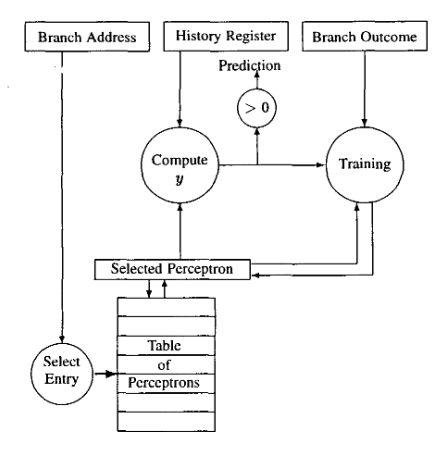
\includegraphics[width=0.5\textwidth]{Chapter1/Figs/perceptron.png}
\caption{\centering Perceptron Predictor Block Diagram\cite{jimenez_dynamic_2001}. }
\label{fig:perceptron2001}
\end{figure} % trace length plot

\newpage
\subsubsection{TAGE}

The history length is a key question for branch predictor. Longer histories enable accurate predictions for some HTP branches while taking more time to warm-up, reducing accuracy for ETP branches. Geometric history length\cite{seznec_analysis_2005} helps find a balance for this question: predictor with shorter history length provides predictions early on before longer predictors finishes warm-up stage. PPM data compression algorithm can be a efficient way to manage and select from predictors with various history length.
\par\hspace*{\fill}\par
TAGE, derived from a PPM-like predictor \cite{michaud_ppm-like_2005} by André Seznec, Pierre Michaud (2006), combines the advantage of geometric history length and PPM data compression algorithm, thus enables more efficient storage of detected patterns.


\subsection{New trends in branch prediction field}

Some new trends and concepts in branch prediction field are briefly mentioned and core reference are cited for future study.

\subsubsection{Security issues}

As the security and privacy of computer systems has become increasingly emphasised, research interest has attracted into the security of branching predictors under side-channel attacks. Side channel attack is based on leaked information from the physical implementation of the cryptosystem rather than theoretical weaknesses in the encryption algorithm. Under this kind of attack, shared directional branch predictor can be manipulated by the attacker and the prediction and  history target can be leaked\cite{evtyushkin_branchscope_2018}. It is difficult for mitigation technique to achieve both performance and isolation, but there are some meaningful attempts\cite{vougioukas_brb_2019}.


\subsubsection{Offline training}

Offline training refers to training of the predictor before the execution of the program and its counterpart is runtime branch prediction. The limited resources on a chip and the low latency requirements limit the scale and complexity of branch prediction algorithms. However, it is possible to improve predictor accuracy by extracting the properties of branch traces in advance for offline training. Offline learning takes place in two main stages: compiling and profiling.

\subsection{Warehouse-scale computer (WSC)} % 1.1.4

In the section, the general idea of WSC is briefly mentioned, followed by emphasising the key features of the WSC that may affect the work of branch predictor. \par\hspace*{\fill}\par

WSCs are a kind of datacenter that provide large-scale, high-performance, low-cost Internet, computing and storage services\cite{barroso_datacenter_2013}. Born out of the demand for large-scale computing for a small amount of applications (e.g. webmail, web search, online translation), in recent years it has gradually taken over a large amount of computing and storage demands that would otherwise have been carried out locally as the price of computing power has fallen. \par\hspace*{\fill}\par

However, WSCs are fundamentally distinct from traditional benchmarks due to the need for on-demand scalability, elasticity and availability. Unlike traditional datacenter where a number of independent and different machines are physically put together, machines in WSC are more homogeneous, emphasising internal connection. Machines often have similar hardware architectures, run on the same software platform, and are connected and managed under the same system management layer. \par\hspace*{\fill}\par

WSCs run a small number of super-scale tasks, usually on thousands of machines simultaneously, flexibly allocating computing power according to demand. Super-scale tasks can have two significant consequences:
\begin{enumerate}[itemsep= 0pt,topsep = 0pt, partopsep=4 pt, leftmargin= 32 pt]
\item Data parallelism arises from large datasets that need to be processed. These large-scale datasets 
often require a large amount of computation for each parallel (sub) task, which may lead to 
periodic, regular instruction streams performed by a single core over a period of time.
\item Executables are also getting bigger. The increased range of instructions makes it harder for 
branch predictors to predict correctly.
In addition, WSC has a greater instruction throughput and typically has a larger reorder window (i.e. 
out-of-order buffer), resulting in a greater reliance on high accuracy branch predictions. However, the 
branch predictor design is not specifically optimised for this critical and unique load.
\end{enumerate}
%********************************** %Second Section  *************************************
\section{Motivations and Objectives} %Section - 1.2

WSC has been in increasing demand and deployment in recent years, and its unique load characteristics are expected to have an impact on branch predictors. Prediction accuracy under such loads has been a gap and is waiting to be investigated. May 2022, google released google datacenter's actual instruction and memory access traces, making research on WSC more feasible and convenient. \par\hspace*{\fill}\par

Here are the main goals of the project. Note that attention is only focused on the directional branch predictors at this stage.\par


\begin{enumerate}[itemsep= 0pt,topsep = 0pt, partopsep=4 pt, leftmargin= 32 pt]
\item (completed) To get familiar with the branch prediction field and compose a well-categorised review of the field, including brief development history, the latest trends and SOTA design.
\item (completed) To setup the required infrastructures on the HUAWEI laptop and server and launch the branch  predictor simulator under default traces. 
\item(completed) To do necessary data processing on Google traces so that it can be accepted by the CBP-5 simulator without losing required information. 
\item(core objective, completed) To evaluate the accuracy of direction prediction vs capacitance of branch predictors (TAGE, perceptron) on Google Workload Traces and compare the results with the prediction accuracy under conventional load.
\end{enumerate}

%********************************** % Third Section  *************************************
\section{Report Organization}  %Section - 1.3 
\label{section1.3}

The report is structured as follows: the second section discusses the method used in the 
simulation. This includes the introduction of simulation infrastructure: CBP-5 simulator kit and Google Workload traces. The method of converting Google WSC traces into CBP-5 BT9 file is also discussed. In the next section, the results of the simulation are presented and discussed in the following order: traces statistic analysis, impact of trace sets on simulation and impact of predictors on simulation results. Some discussion about the conduct on the project is also made in this section. Finally, conclusions are drawn based on the current progress.




%!TEX root = ../thesis.tex
%*******************************************************************************
%****************************** Second Chapter *********************************
%*******************************************************************************

\chapter{Methodology}

The core task of the project is to investigate the prediction accuracy of directional branch predictors
under WSC workload. To achieve this, WSC branch traces that fit real-world WSC load scenarios are 
needed, and a sufficiently efficient and well-accepted simulator is required to make the result 
convincing, not to mention a high-performance platform to provide the computing resources.

This section demonstrates where and how the the experiment are implemented.

\ifpdf
    \graphicspath{{Chapter2/Figs/Raster/}{Chapter2/Figs/PDF/}{Chapter2/Figs/}}
\else
    \graphicspath{{Chapter2/Figs/Vector/}{Chapter2/Figs/}}
\fi

\section{Simulation infrastructure}

\subsection{5th Branch Prediction Championship (CBP-5) Kit}

CBP-5 \cite{noauthor_championship_nodate} is a conditional branch predictor simulator provided by Branch Prediction Championship, a competition organised by \textit{The Journal of Instruction-Level Parallelism}. Since the first competition was held in 2004, CBP has gradually become a widely accepted branch predictor simulator. \par\hspace*{\fill}\par

There are several reasons why CBP-5 is very well suited to this project. Firstly, it is speedy. Unlike 
Gem5, QEMU and other whole-chip simulation tools, CBP-5 focuses on the directional branch 
predictors' simulation and is implemented in C++, thus can simulates far faster than Gem5 and QEMU. Secondly, its simplicity reduces potential hurdles when being applied to other trace formats (e.g. Google Workload Traces). The smooth learning curve also makes it more suitable for this time-critical project. Finally, there are useful branch instruction traces (223 training traces) and SOTA predictors (winner submission of the competition) attached to this simulator kit and can help streamline project workload.

\subsubsection{CBP-5 traces}
223 traces are given in the CBP-5 kit and separated into four catagories: 19 long mobile traces, 61 short mobile traces, 4 long server traces and 139 short server traces. Long traces have 1 billion instructions and shot traces have 100 million instructions. In this project we combine all 80 mobile traces as CBP-5 \textit{mobile} trace set, and all 143 server traces as CBP-5 \textit{server} trace set.

\subsubsection{CBP-5 predictors}
11 prize-winning predictors are given in the CBP-5 kit, including SOTA \textbf{TAGE-SC-L}\cite{seznec_tage-sc-l_2016} (8KB \& 64KB), \textbf{MTAGE+SC}\cite{seznec_exploring_2016} (Unlimited size),\textbf{ Multiperspective Perceptron Predictor}\cite{jimenez_multiperspective_2016} (8KB, 64KB \& Unlimited), \textbf{Multiperspective Perceptron Predictor with TAGE}\cite{jimenez_multiperspective_2016-1} (8KB, 64KB \& Unlimited) and \textbf{Dynamically Sized TAGE}\cite{pruett_dynamically_2016} (8KB \& 64KB). All predictors are simulated but the discussion on predictors is focused on TAGE-SC-L, MTAGE-SC and Multiperspective Perceptron with TAGE.

\subsubsection{CBP-5 trace format: BT9}
CBP-5 uses \textit{Branch Trace version 9} (BT9) as its input file format. A complete branch instruction trace is translated into the a flow control graph (e.g. Figure~\ref{fig:branch graph}) and its node table, edge table and edge sequence are stored in a BT9 file, therefore being a space-saving format.

\begin{figure}[h!] 
\centering    
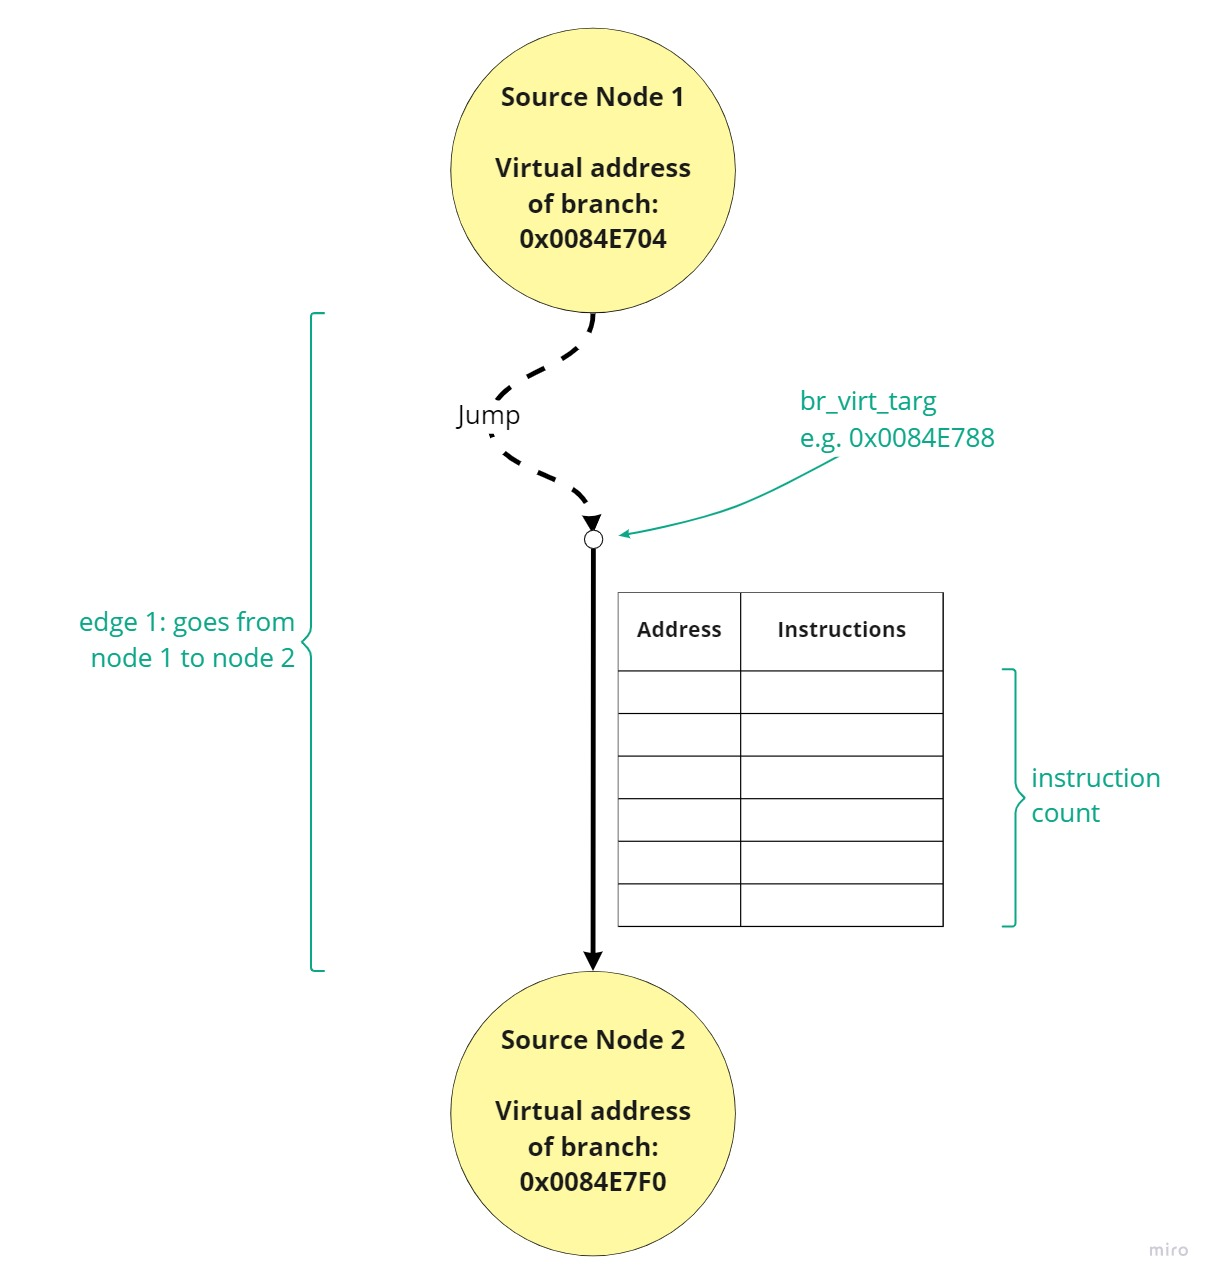
\includegraphics[width=0.5\textwidth]{Chapter2/branch graph.jpg}
\caption{\centering BT9 format example: control flow graph}
\label{fig:branch graph}
\end{figure} 


\subsection{Google workload traces}
Released May 2022, the Google Workload Traces\cite{noauthor_google_nodate} project is driven by the rapid growth of warehouse-scale computers (WSCs) in today's computing market and hopes to improve research in the WSC architecture by sharing real WSC workload data. The traces are captured from Google datacentre using \textit{DynamoRIO}'s \textit{drmemtrace}, including instruction and memory address traces (.memtrace.gz) as well as branch traces (branch\_trace.<tid>.csv.gz). Each representing a unique WSC application, there four trace folders named \textit{delta}, \textit{whiskey}, \textit{charlie} and \textit{merced}. All traces inside a folder are captured in a single launch thus sharing virtual address space.\par\hspace*{\fill}\par

As the first published WSC traces, Google workload traces fit well with this project by offering a domain 
different from all traditional benchmarks. At the stage the focus is on the branch traces.


\subsection{Computing platform}

The simulation is power by a HUAWEI server equipping two Intel(R) Xeon(R) Gold 6161 CPUs and 
supporting a maximum of 88 threads. Computing resource is accessed by SSH, and a Docker container 
is created on the server to provide a safe working environment. All simulation data is analysed by \textit{numpy} and plotted by \textit{matplotlib}. 



\section{BT9 Format conversion}
\label{BT9 Converson}

This section stems from the mismatch between the CBP-5 and WSC branch trace formats; CBP-5 uses the BT9 format, while WSC traces are captured by DynamoRIO and therefore use the DynamoRIO format. There are two potential solutions to the mismatch, either designing a program that converts Google WSC traces into BT9 format or modifying the frontend part of CBP-5. The former option is taken in this project, beacuse designing a program that only formats the WSC trace would make the risk more manageable than modifying the simulator with thousands of lines of code. Besides, modified CBP-5 may reduce the acceptance of the results. \par\hspace*{\fill}\par

This is one of the core objectives of the project and takes the major project period. Since a WSC trace is structured as a sequential branch instruction list while a BT9 file is stored as node table (unique branches), edge table and edge sequence (abbreviated branch instructions), the foundamental idea of conversion is simple: read branch instruction one by one trace file, update the node table and edge table, and then append the interpreted edge into edge sequence. \par\hspace*{\fill}\par

However, because of the mismatched information, some unexpected problems were encountered during the conversion leading to a one-week delay.


\subsubsection{Behaviour, size and instruction count}
Though the behaviour information is expected in BT9 format, it is not used in the predictor. Thus we block the behaviour entry in BT9. \par\hspace*{\fill}\par

Instruction count refers to the number of non-branch instructions executed between two branch instructions. Whatever instruction size is used in the calculation, some instruction count are fractions or negative numbers. The invalid instruction count implies that in contrast to the fixed-size instructions in the CBP-5 traces, instructions in Google WSC traces have various sizes (and is presumed to be x86\_64 instruction set)

\subsubsection{Branch type conversion}

The classification of branch types in two formats are different. In BT9, each branch must take a label from each of the following classes:

\begin{description}[itemsep= 0pt,topsep = 0pt, partopsep=4 pt, leftmargin= 32 pt,labelindent=32pt]
\item[Type] \qquad\qquad\qquad Return, Jump, Call
\item[Directness] \qquad\qquad DIRECT, INDIRECT
\item[Conditionality] \qquad CONDITIONAL, UNCONDITIONAL
\end{description}

\hspace*{\fill}\par
However in Google WSC traces, branches are categorised into eight types, as shown in the first column of Table~\ref{table:branch type}. Obviously, the conversion cannot be done directly, and three problems are listed below.

\begin{enumerate}[itemsep= 0pt,topsep = 0pt, partopsep=4 pt, leftmargin= 32 pt]
\item No Google branch types are specified the Conditionality except \textit{conditional jump}

Based on an observation that all branches in Google WSC traces are 100\% taken except \textit{conditional jump}, it is assumed that all other types are unconditional.


\item The \textit{interrupt} and \textit{context switch} do not correspond to any of the BT9 label. \label{interrupt}

This problem indeed exists and cannot be address directly. However, noting that only a tiny fraction of branch instructions are \textit{interrupt} or \textit{context switch} (verified in Section~\ref{frantion of interrupt}), they are ignored in this project by being converted into JMP+DIR+UND, a common and undirectional type that won't affect conditional branch predictors. 

\item The \textit{conditional jump} has no clear Directness

Because the project studies the condition branch predictor only (i.e. predict taken or not-taken), the directness does not affect the simulation results. \textit{conditional jump} interpreted as DIRECT branch because direct branches are the majority of all branches.

\end{enumerate}



\begin{table}
\centering
\begin{tabular}{c c c}
\toprule{\LARGE}
Google WSC type & BT9 type & \textit{problem encountered} \\ 
\cmidrule{1-3}

\textit{direct call}         &   CALL+DIR+UCD    &1\\
\textit{indirect call}       &   CALL+IND+UCD    &1\\
\textit{direct jump}         &   JMP+DIR+UCD     &1\\
\textit{indirect jump}       &   JMP+IND+UCD     &1\\
\textit{conditional jump}    &   JMP+DIR+CND     &3\\
\textit{return}              &   RET+IND+UCD     &1\\
\textit{interrupt}           &   JMP+DIR+UCD     &2\\
\textit{context switch}      &   JMP+DIR+UCD     &2\\

\bottomrule
\end{tabular}
\caption{\centering \small Branch type conversion result}
\label{table:branch type}

\end{table} % branch type table







\nomenclature[z-WSC]{WSC}{Warehouse-Scale Computer}
\nomenclature[z-BT9]{BT9}{Branch Trace version 9, a trace format applied by CBP-5}
\nomenclature[z-MPKI]{MPKI}{Misprediction Pre 1K Instructions}
\nomenclature[z-HTPB]{HTPB}{Hard To Predict Branch}
\nomenclature[z-UDUB]{UDUB}{UniDirectional Unique Branch}
\nomenclature[z-TAGE]{TAGE}{TAgged GEometric history length branch prediction}


\nomenclature[z-PHT]{PHT}{Pattern History Table}
\nomenclature[z-ETPB]{ETPB}{Easy To Predict Branch}
\nomenclature[z-UB]{UB}{Unique Cranch}
\nomenclature[z-PC]{PC}{Program Counter}
\nomenclature[z-PPM]{PPM}{Prediction by Partial Matching}
\nomenclature[z-MPP]{MPP}{Multiperspective Perceptron Predictor}
\nomenclature[z-DS-TAGE]{DS-TAGE}{Dynamically Sized TAGE}

\nomenclature[z-MPP]{MPP-TAGE}{Multiperspective Perceptron Predictor with TAGE}


\nomenclature[x-a]{\textit{Set of trace / trace set}}{
There are six sets of traces: CBP-5 \textit{mobile}, \textit{server}, Google WSC \textit{delta}, \textit{whiskey}, \textit{charlie}, \textit{merced}. Set is the basic unit for the simulation and calculation in the project. For WSC, set is also the maximum range in which traces are captured under same launch and share virtual address space.
}

\nomenclature[x-b]{\textit{\textit{Unique Branch }}}{
Unique branch (UB) is defined inside a set for WSC traces and a trace for CBP-5 traces. Unique branch represents the branch instructions stored in same virtual address. An branch in an virtual address can only be counted as one unique branch no matter how many times it is executed.
}


\nomenclature[x-c]{\textit{\textit{Branch Instruction}}}{Branch instruction is the concept opposite to unique branch. If a unique branch is executed 10 times, the number of branch instructions is counted as 10, though the number of unique branch is always one.}

%!TEX root = ../thesis.tex
%*******************************************************************************
%****************************** Third Chapter **********************************
%*******************************************************************************
\chapter{Results}

% **************************** Define Graphics Path **************************
\ifpdf
    \graphicspath{{Chapter3/Figs/Raster/}{Chapter3/Figs/PDF/}{Chapter3/Figs/}}
\else
    \graphicspath{{Chapter3/Figs/Vector/}{Chapter3/Figs/}}
\fi

% Talk about ... in this section
This section presents the results of the simulation and gives some analysis and discussion about the results. An analysis of the trace statistics is given first, including trace lengths and trace composition (conditional branches and single-direction branches). Immediately afterwards the simulation results are compared between the trace sets and some useful WSC trace features are obtained, inspiring some thoughts on the causes of the prediction accuracy under the WSC workload. In the third section TAGE\cite{seznec_tage-sc-l_2016, seznec_exploring_2016} (SOTA) and some other predictors \cite{pruett_dynamically_2016, jimenez_multiperspective_2016-1, jimenez_multiperspective_2016} are compared. Finally, a review of the completion of the project is given and limits are discussed in detail.

% Section 3.1 Trace stat
\section{Traces statistics}

When studying new trace sets, it is natural and necessary to first study the statistical properties of the sets themselves. The four WSC sets (\textit{delta, whiskey, charlie} and \textit{merced}) show significant differences from each other, indicating that WSC workload branch traces strongly depend the application run on WSC.


\begin{figure}[h!] 
\centering    
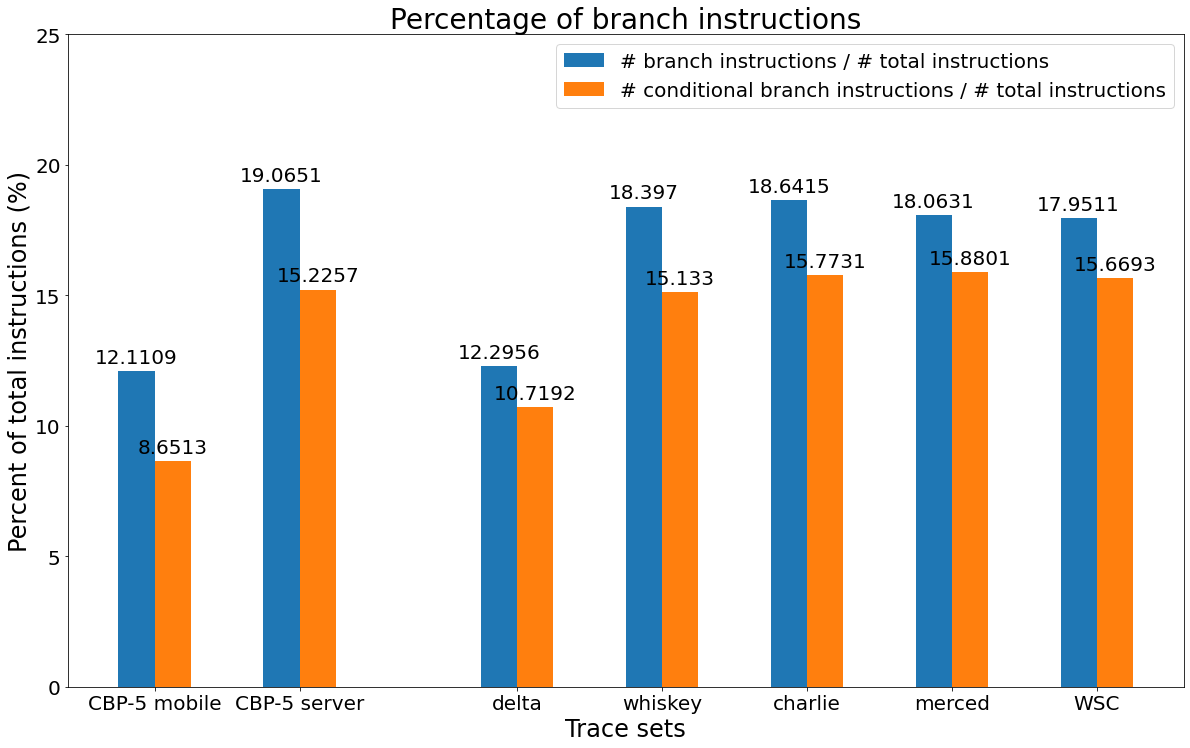
\includegraphics[width=0.8\textwidth]{Chapter3/Figs/br percent.png}
\caption{\centering Branch instruction and conditional branch instruction percent}
\label{fig:branchinstfrac}
\end{figure} % branch inst fraction plot


\subsubsection{Fraction of branch instructions}

As this project focused on conditional branch only, the proportions of branch instruction and conditional branch instructions are studied first Figure~\ref{fig:branchinstfrac}. The proportions of both branch instructions and conditional branch instructions in WSC sets are almost equal to those in CBP-5 \textit{server} and higher than in CBP-5 \textit{mobile}, suggesting a higher similarity between WSC and CBP-5 \textit{server} than CBP-5 \textit{mobile}. Also note that \textit{delta} have fewer branch instructions and conditional branch instructions than other WSC sets, which is one of the major causes why \textit{delta} has the smallest MPKI among the WSC sets. \par\hspace*{\fill}\par



Besides, 0.00127\% instructions are \textit{interrupt} and 0.00142\% instructions are \textit{context switch} in WSC sets.
This verifies the previous assumption in Section~\ref{interrupt} that \textit{interrupt} and \textit{context switch} take small proportion of the sets and that ignoring them has a negligible effect on the simulation results.
\label{frantion of interrupt}

\subsubsection{Trace lengths}

\begin{figure}[h!] 
\centering    
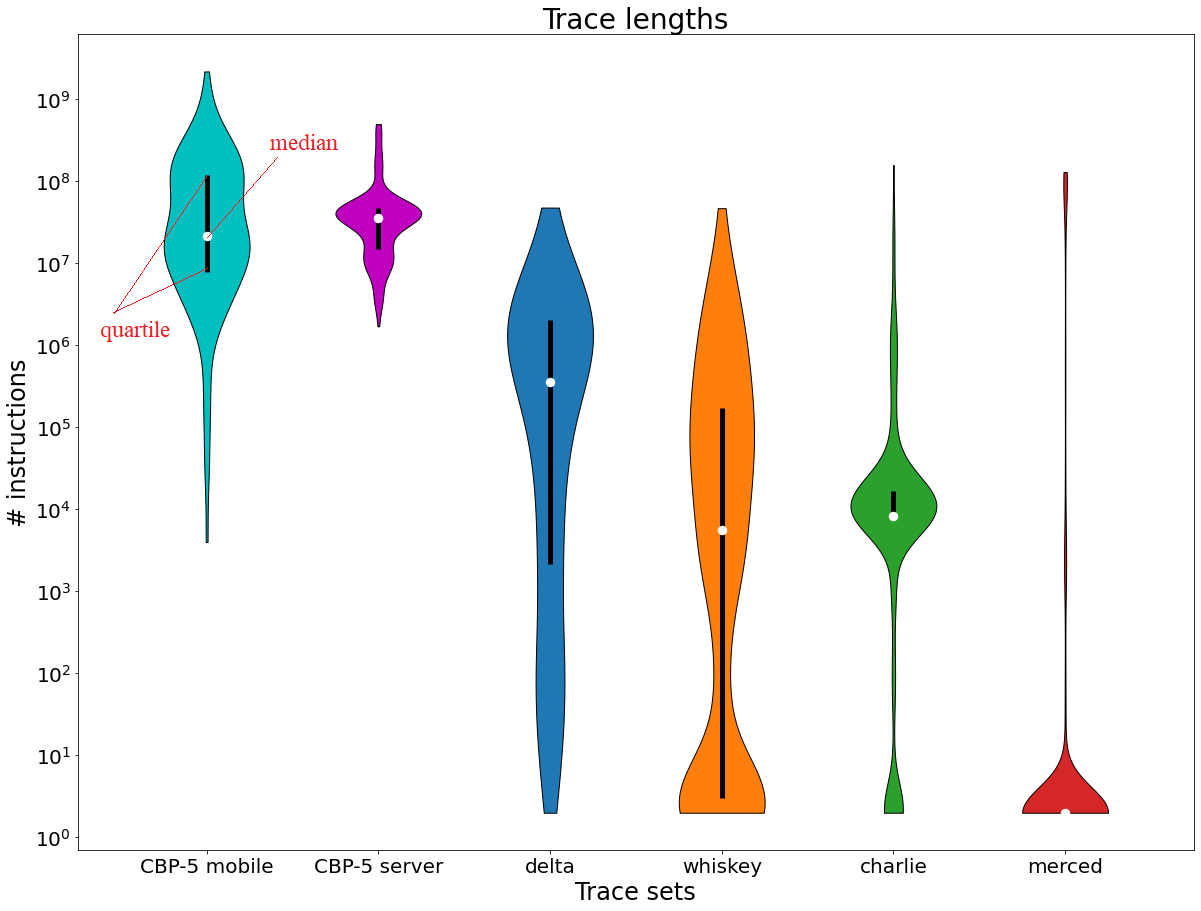
\includegraphics[width=0.8\textwidth]{Chapter3/Figs/tracelength.png}
\caption{\centering Trace lengths of six trace sets}
\label{fig:tracelength}
\end{figure} % trace length plot

In this report, since both CBP-5 and WSC traces show similar proportions of branch instruction, trace length is defined as the number of all types of instructions in a trace. Figure~\ref{fig:tracelength} shows the trace length distribution of each trace set, where the vertical coordinates indicate the trace length and each violin plot represents a set, with wider indicating more traces locate at the corresponding length.\par\hspace*{\fill}\par

While 90\% CBP-5 traces longer than $10^6$ instructions, WSC traces are significantly shorter and less concentrated with many traces even shorter than 100 instructions (particularly \textit{whiskey} and \textit{merced}). Since Google Workload Traces\cite{noauthor_google_nodate} are raw data directly captured from the machine and each trace represents a software thread, we presume very short traces represent idle threads while the program is running. As the predictors require a learning process, too short traces do not reflect the prediction accuracy of the predictor, and an example is thousands of traces containing only 16 instructions reporting an MPKI of 62.5, well above the MPKI reported by other long traces. 

\subsubsection{Uniting traces}

Since short traces contribute unreasonably high MPKIs but have very limited impact on actual system performance, the default methods of CBP-5 that counts the MPKI of all traces and calculate the arithmetic mean for each set is no longer reasonable for Google Workload Traces. Three new solutions were proposed to overcome this problem: 

\begin{enumerate}[itemsep= 0pt,topsep = 0pt, partopsep=4 pt, leftmargin= 32 pt]
\item Filter traces shorter than a certain length 
\item \textbf{Unite all the traces in a set after the simulation. }
\item Do not reset the predictor between traces in the same set.
\end{enumerate}

\hspace*{\fill}\par
Confirmed with Google, this solution 2 is supported by the fact that all traces within the same trace set are for the same run of the application, therefore share the address space. In a set if two branches occurring in different traces share same virtual address they are recognised as same unique branch, thus the total executed number and misprediction number within a set can be obtained for each unique branch, and this is called "uniting traces" in this report. In solution 2, each trace is still simulated independently and the MPKI is calculated after uniting the simulation results of all the traces in a set. Solution 1 requires a reasonable criteria to filter traces which we do not currently have and solution 3 is time consuming, requiring additional code and another simulation. Given the limited project duration, solution 2 is applied and WSC traces are united within each sets.\par\hspace*{\fill}\par

One of the idea raised from uniting WSC traces is can CBP-5 traces also be united? This idea is objected by Table~\ref{table:unite CBP}, whose first row represents the number of UBs in each set and second row is obtained directly adding up the number of UBs in each individual trace). The third row shows the ratio of the first row to the second row, it is called commonality ratio and it reflects the proportion of branches that are shared by different traces within a set; the lower the commonality ratio, the more likely it is that the set of traces was captured under a single launch. Both CBP-5 sets have a much higher commonality ratio than WSC traces, implying that they are less likely captured under same software launch.\par\hspace*{\fill}\par

Comparing the united mean of WSC sets with the arithmetic mean of CBP-5 may be questioned to be unscientific. However, the CBP-5 traces are parallel and independent with each other so it is logically to calculate their arithmetic mean; whereas the traces in a WSC set are captured under a single launch, contain complex interconnections and are not equivalent (some threads carry the main workload) so it is reasonable to introduce weight by uniting traces.

\begin{table}[h!] 
\centering
\begin{tabular}{l r r r r r r}
\toprule{\LARGE}
\multirow{2}{*}{} & \multicolumn{2}{c}{CBP-5} & \multicolumn{4}{c}{Google Workload Traces} \\ 
\cmidrule{2-3} \cmidrule{4-7}
  & \textit{mobile} & \textit{server}  & \textit{delta} & \textit{whiskey} & \textit{charlie} & \textit{merced}  \\ 
\midrule
\# unique branches (UBs)     & \sout{152K}   & \sout{456K}  & 63K  & 904K  & 499K & 290K  \\

\# adding up UBs  & 444K   & 2,234K  & 1,088K  & 10,481K  & 20,035K  & 56,328K \\

commonality ratio         & 34.3\% & 20.4\%  & 5.81\% & 8.63\%  & 2.49\%  & 0.515\% \\

\# average UBs (top 6) & 35.5K & 82.7K & 23.0K & 166.5K & 282.1K & 133.1K \\

\bottomrule
\end{tabular}
\caption{\centering \small Commonality reatio \& Average UBs (top 6). The commonality ratio reflects the proportion of branches that are shared by different traces within a set; the lower the ratio, the more likely it is that the set of traces was captured under a single launch.}
\label{table:unite CBP}
\end{table} % Uniting trace verification

\subsubsection{Number of unique branches (UBs)}

The reason for the interest in the number of UBs is because of Aliasing. Aliasing is a well-known phenomenon that affects predictor accuracy by limiting the predictor's ability to accurately identify UBs. Due to the limited capacity of the predictor, a great amount of UBs in a trace can put high pressure on the predictor capacity, thus causing aliasing and reducing predictor accuracy.\par\hspace*{\fill}\par

Considering the large number of short traces in WSC sets, the average of the six traces with the most UBs are calculated and appended to Table~\ref{table:unite CBP}. According to the averaged UBs, \textit{server} has two times more than \textit{mobile}, in line with the simulation results where the MPKI of \textit{server} is more than twice that of the \textit{mobile}. Most WSC traces (i.e. except \textit{delta}) have 1.6-3.4 times more UBs than \textit{server}, implying a much higher MPKI than \textit{server} can be expected (though this is not the case, as discussed in Section~\ref{MPKI results}). \par\hspace*{\fill}\par

As to \textit{delta}, not like other WSC sets, it has less UBs than \textit{mobile}, implying that its MKPI can be even lower than mobile (verified by the simulation result). Besides, the great variation between WSC applications is again confirmed: delta looks more like \textit{mobile} than a WSC set.


\subsubsection{Fraction of unidirectional unique (UU) branches}

Unidirectional unique branches (UDUBs) are of particular interest because they have only one choice (T or N) and are easy to predict while occupying the same amount of resources as other more complex UBs under the present predictor schemes. Research on them may help optimize predictor designs for UU branches to saving valuable capacity. Since uniting is not valid for CBP-5 sets, six traces with the largest number of UBs are selected and averaged (Table~\ref{table:selected CBP-5}) for both CBP-5 \textit{mobile} and CBP-5 \textit{server}. The fraction of taken UU branches, not-taken UU branches, their summation and the ratio of taken UU branches to not-taken UU branches are obtained for selected CBP-5 traces and united WSC sets.

\begin{table}[h!] 
\vskip 0.2in
\centering
\begin{tabular}{c c c c c c}
\toprule{\LARGE}
\multirow{2}{*}{} & \multicolumn{2}{c}{\textit{mobile}} & \multicolumn{2}{c}{\textit{server}} &\\ 
\cmidrule(l{3pt}r{3pt}){2-3} \cmidrule(l{3pt}r{3pt}){4-5}
&trace name & \# UBs & trace name & \# UBs  \\ 
\midrule
&SHORT\_MOBILE-33 & 41984 & SHORT\_SERVER-5 & 89864\\
&LONG\_MOBILE-14 & 38832 & LONG\_SERVER-2.res & 89864\\
&SHORT\_MOBILE-32 & 36949 & SHORT\_SERVER-6.res & 88689\\
&SHORT\_MOBILE-35 & 33592 & LONG\_SERVER-3.res & 88689\\
&SHORT\_MOBILE-36 & 30839 & SHORT\_SERVER-8 & 69612\\
&LONG\_MOBILE-15 & 30839 & LONG\_SERVER-4.res & 69612\\
\bottomrule
\end{tabular}
\caption{\centering \small Selected CBP-5 traces with the largest number of unique branches (UBs)}
\label{table:selected CBP-5}
\end{table} % Table: selected CBP-5


It's clearly shown in Table~\ref{table:UU Branches} that the fraction of UU branches are similar and about 80\% for both CBP-5 and WSC, hinting at the potential for optimisation for UU branches. Whoever the ratio of taken UU branches to not-taken UU branches are significantly different in CBP-5 and WSC. Depending on different WSC sets not-taken UU branches can be 5~12 times more than taken UU branches, compared with 1.5 times for \textit{mobile} and 2.1 times for \textit{server}. More not-taken UU branches indicate that WSC is a stronger biased workload, which reduces the direction prediction difficulty. Another point worth mentioning is that the WSC still show significant differences about UU branches between sets: \textit{merced} has the smallest proportion of UU branches while \textit{whiskey} has the largest.\par\hspace*{\fill}\par


In contrast to UU branches, hart-to-predict (HTP) branches are also of interest and are discussed this in later sections.

\begin{table}[h!] 
\centering
\vskip 0.2in
\begin{tabular}{l r r r r r r}
\toprule{\LARGE}
\multirow{2}{*}{} & \multicolumn{2}{c}{CBP-5} & \multicolumn{4}{c}{Google Workload Traces} \\ 
 \cmidrule(l{3pt}r{3pt}){2-3} \cmidrule(l{3pt}r{3pt}){4-7}
  & \textit{mobile} & \textit{server}  & \textit{delta} & \textit{whiskey} & \textit{charlie} & \textit{merced}  \\ 
\midrule
Taken UU branches      & 30.42\%   & 25.90\%    & 6.25\%  & 12.31\%  & 9.38\%   & 6.43\% \\

Not-taken UU branches   & 46.40\%   & 54.39\%  & 73.51\%  & 70.16\%  & 68.44\%  & 62.10\% \\

All UU branches         & 76.82\%   & 82.83\%  & 79.75\%  & 82.46\%  & 77.82\%  & 68.53\% \\

Not-taken / Taken         & 1.536     & 2.101    & 11.77    & 5.700    & 7.298    & 9.653   \\
\bottomrule
\end{tabular}
\caption{\centering \small Fraction of unidirectional unique branches (UDUBs). CBP-5 data is obtained from six selected traces, while WSC data is obtained from united WSC sets.}
\label{table:UU Branches}
\end{table} % Table: UU Branch


\section{Impact of trace sets on MPKI}

The simulation results are discussed in this section, mainly around the differences between trace sets. Despite the high pressure put on the predictors' capabilities by the large number of UBs, the WSC sets reports MPKIs that are similar to or even slightly lower than the MPKI of \textit{server}. This result means that due to specific tasks and similar context\cite{barroso_datacenter_2013} WSC is a more predictable workload. Note that WSC sets continue to show a huge variation in simulation results, emphasising the importance of application-specific analysis.\par\hspace*{\fill}\par

The MPKI are shown in Figure~\ref{fig:MPKI}. Contrary to previous expectation, MPKI of united WSC is 15.7\% lower than server, suggesting that there are other factors increase WSC prediction accuracy (e.g. very few applications or large fraction of not-taken UDUBs). Since WSC sets are highly differentiated, all sets are shown in Figure~\ref{fig:Normalized MPKI}. Normalizing sets to server is to compare the adaptability of different predictors to WSC in later section. MPKI proves that \textit{whiskey, charlie} and \textit{merced} put higher pressure on predictor capacity than \textit{delta}, due to much more UBs.\par\hspace*{\fill}\par


The paradox of WSC sets (except \textit{delta}) having more UBs but lower MPKI than \textit{server} suggests that WSC has some features makes branches highly predictable, which is in line with previous summaries of WSC features from a higher level. Despite WSC sets have more UBs, they also have more not-taken UUBs (thus strongly biased), more specific application and larger-scale parallel instruction context. \par\hspace*{\fill}\par

\begin{figure}[h!] 
     \centering
     \begin{subfigure}{1\textwidth}
         \centering
         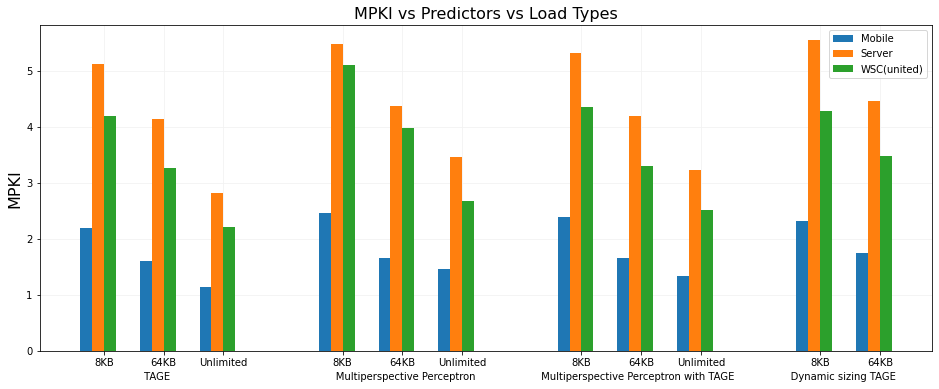
\includegraphics[width=1.0\textwidth]{Chapter3/Figs/MPKI vs Predictors vs Load Types.png}
         \caption{MPKI vs Predictors vs Load Types}
         \label{fig:MPKI}
     \end{subfigure}
     \newline
     \begin{subfigure}{1\textwidth}
         \centering
         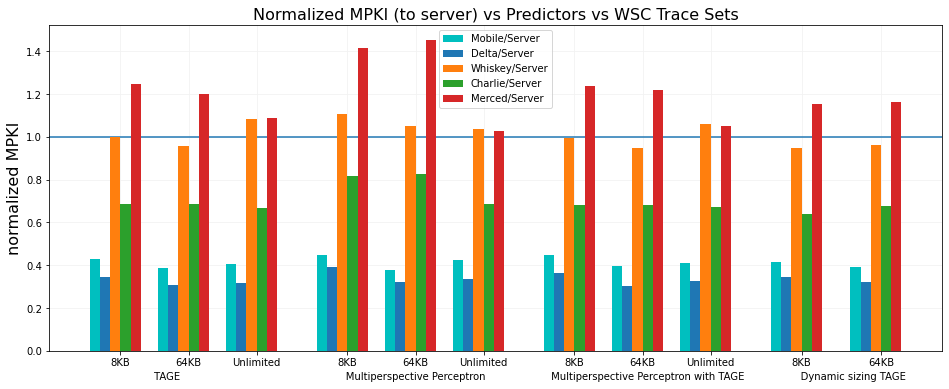
\includegraphics[width=1\textwidth]{Chapter3/Figs/Normalized MPKI (to server) vs Predictors vs WSC Trace Sets.png}
         \caption{Normalized MPKI (to server) vs Predictors vs WSC Trace Sets}
         \label{fig:Normalized MPKI}
     \end{subfigure}
        \caption{MPKI histograms \& Normalized MPKI of 6 trace sets and 11 predictors }
        \label{fig:MPKI histograms}
\end{figure} % MPKI plot
\label{MPKI results}



\newpage
% Section 3.3 Simulation results between predictors % Section 3.2 Simulation results between sets
\section{Impact of predictors on MPKI}

Figure~\ref{fig:MPKI histograms} shows MPKI of all predictor. On WSC sets, TAGE scheme (TAGE-SC-L \& MTAGE-SC) is still SOTA, followed by the Multiperspective Perceptron Predictor with TAGE (MPP-TAGE) and Dynamically sized TAGE (DS-TAGE). The multiperspective perceptron predictor (MPP) reports highest MPKI on all capacities. While DS-TAGE reports higher MPKI than MPP on \textit{server}, DS-TAGE reversed the results on WSC. This draws attention to the variation of each predictor in server and WSC, thus that the normalized MPKI is plotted. 8KB \& 64KB MPP has the largest normalised MPKI and worst adaptation on WSC, resulting in the highest MPKI. However, Unlimited MPP has the smallest normalised MPKI, suggesting that large MMP has the potential to do well on WSC traces. Besides, For all predictors schemes and most WSC sets, unlimited versions report smaller normalised MPKI, because the impact of UBs increasing is less significant for unlimited capacity.


\section{Hard-to-predict branches (HTPB)}

Hard-to-predict branches are those unique branches that hard to predict and contribute to the most of misprediction. By sorting unique branches using the number of mispredictions and ploting the accumulated misprediction percent, Figure~\ref{fig:HTP branches vs WSC sets} are plotted. A horizontal line is placed at 90\% mispredictions to help count how many unique branches contribute 90\% mispredictions to the whole set. This number is defined as the number of HTPB in this project. Four predictors are selected such that three of them are TAGE with different size, and one of them is 64KB MPP-TAGE to campare with 64KB TAGE-SC-L.\par\hspace*{\fill}\par

Firstly, significant variation is still observed for four WSC sets. The number of HTPB generally increase with number of UUBs, but still affected by specific feature of individual set. The more HTPB there are in a set, the larger capacity is required to address those HTPB.\par\hspace*{\fill}\par

Secondly, the numbers of HTPB do not change significantly with predictors, but are suddenly reduced when unlimited capacity is applied. This indicates how many unique branches are hard to be predicted by the current scheme, ignoring the limitation from the predictor size.


\begin{figure}[h!] 
     \centering
     \begin{subfigure}{0.45\textwidth}
         \centering
         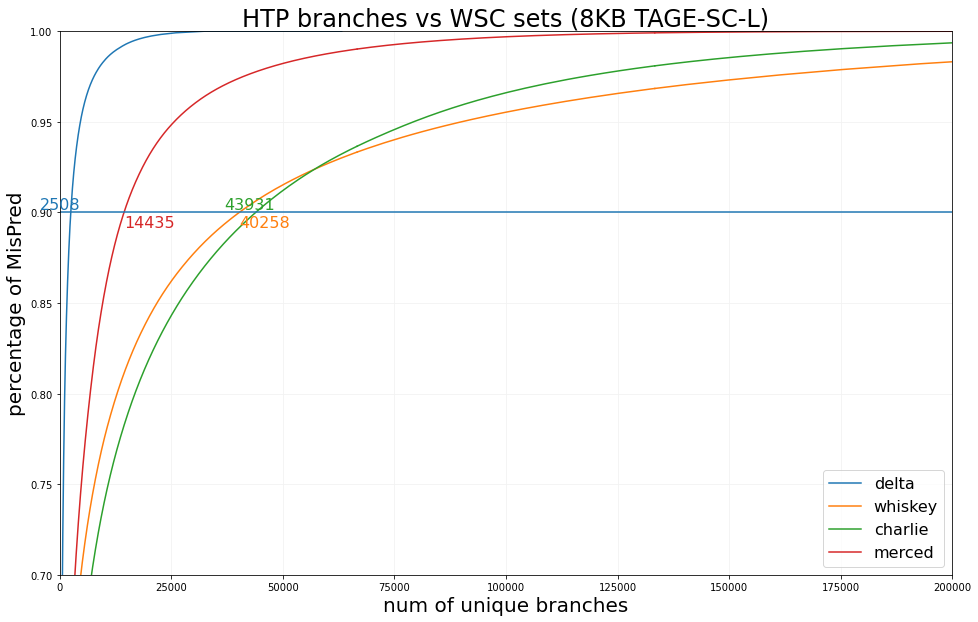
\includegraphics[width=1\textwidth]{Chapter3/Figs/HTP branches vs WSC sets (8KB TAGE-SC-L).png}
         \caption{8KB TAGE-SC-L}
         %\label{fig:MPKI}
     \end{subfigure}
     \begin{subfigure}{0.45\textwidth}
         \centering
         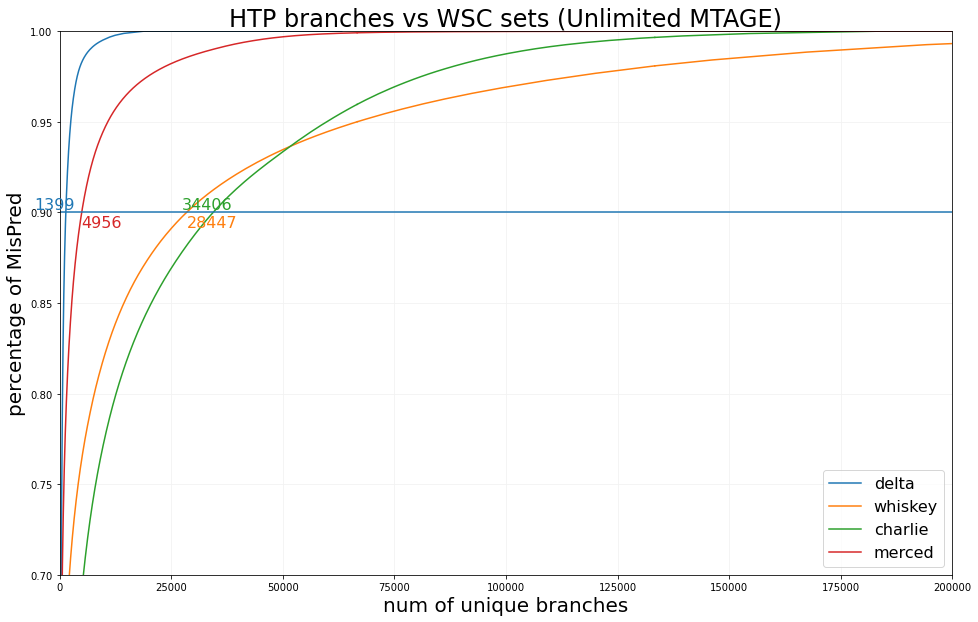
\includegraphics[width=1\textwidth]{Chapter3/Figs/HTP branches vs WSC sets (Unlimited MTAGE) (2).png}
         \caption{Unlimited MTAGE-SC}
         %\label{fig:MPKI}
     \end{subfigure}
     \hfill
     \begin{subfigure}{0.45\textwidth}
         \centering
         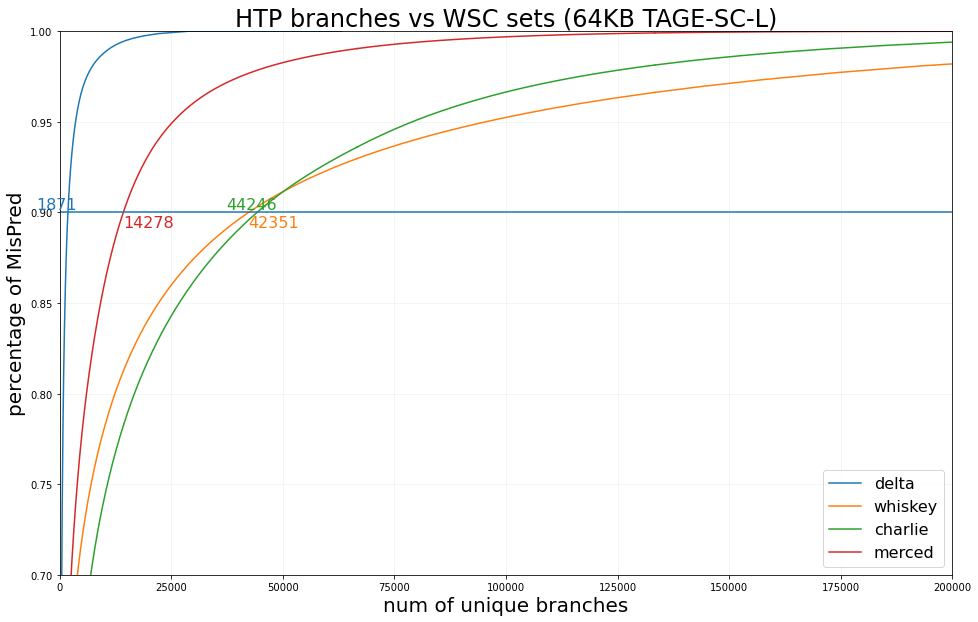
\includegraphics[width=1\textwidth]{Chapter3/Figs/HTP branches vs WSC sets (64KB TAGE-SC-L).png}
         \caption{64KB TAGE-SC-L}
         %\label{fig:Normalized MPKI}
     \end{subfigure}
     \begin{subfigure}{0.45\textwidth}
         \centering
         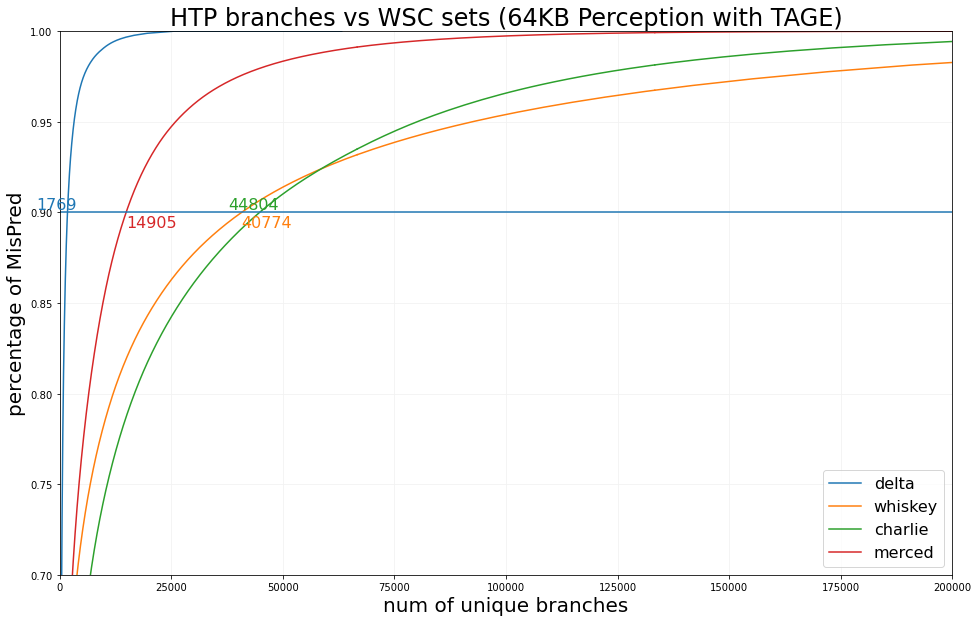
\includegraphics[width=1\textwidth]{Chapter3/Figs/HTP branches vs WSC sets (64KB Perception with TAGE).png}
         \caption{64KB Perception with TAGE (MPP-TAGE)}
         %\label{fig:Normalized MPKI}
     \end{subfigure}
     
\caption{HTP branches vs WSC sets}
\label{fig:HTP branches vs WSC sets}
\end{figure} % MPKI plot
\label{MPKI results}

\newpage
\section{Discussion of the results}
\label{result discussion}

\begin{figure}[h!] 
\centering    
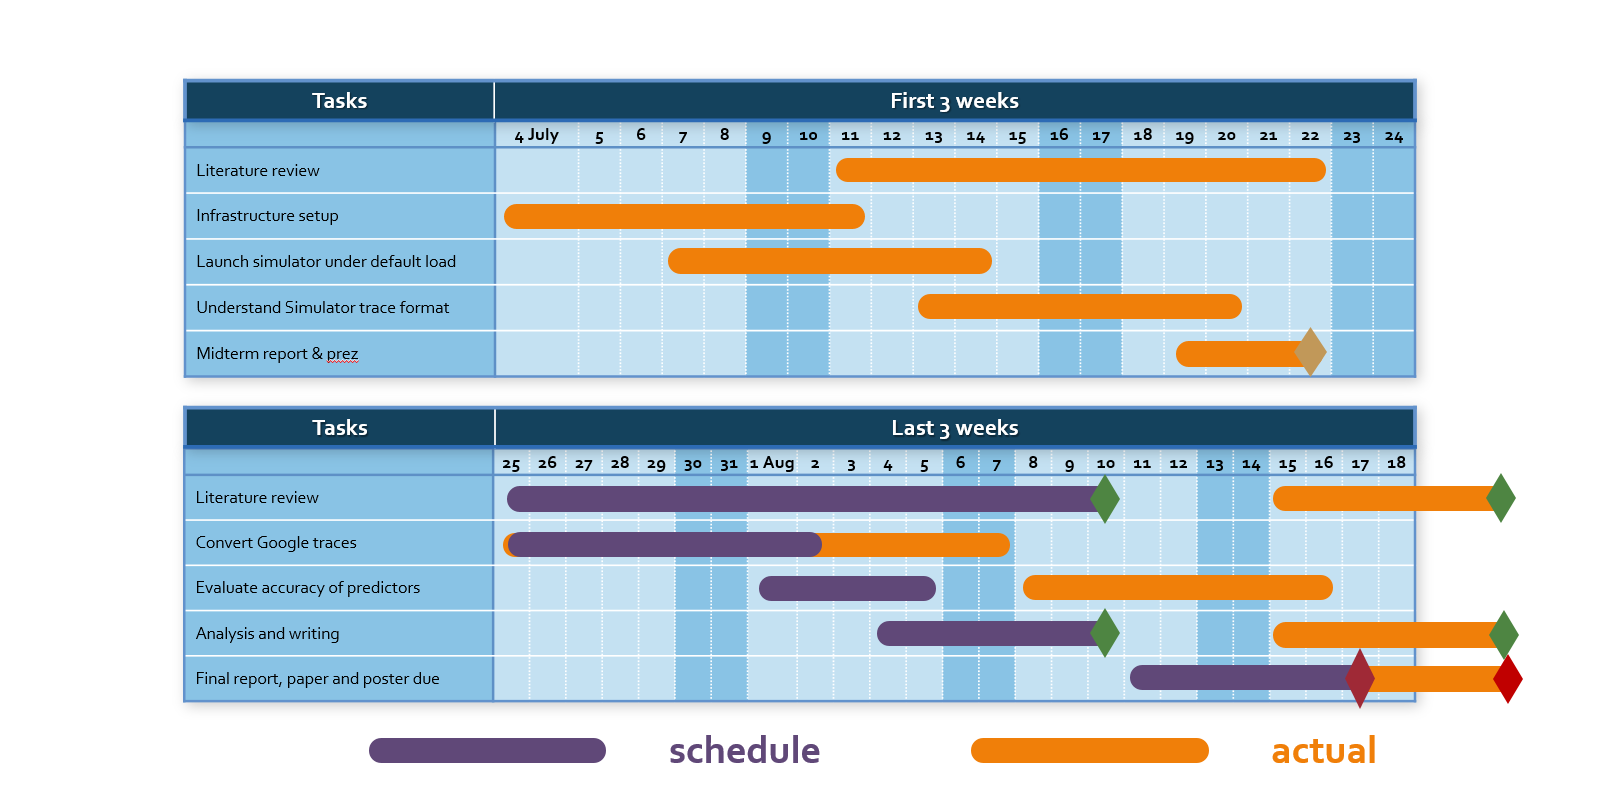
\includegraphics[width=1\textwidth]{Chapter3/Figs/final gantt chart.png}
\caption{\centering Project progress Gantt Chart}
\label{fig:gantt chart}
\end{figure}

Shown in the final gantt chart (Figure~\ref{fig:gantt chart}), the results of the project are generally acceptable and all planned objectives have been completed. Unexpected problems were encountered in two main areas, resulting in delays of the project:

\begin{enumerate}[itemsep= 0pt,topsep = 0pt, partopsep=4 pt, leftmargin= 32 pt]
\item Mismatch between the information provided by Google Workload Traces and expected by CBP-5 simulator.
\item Raw, unprocessed trace sets from Google Workload Traces.
\end{enumerate}

\hspace*{\fill}\par
Problems caused by the former include type, behaviour and size problem as discussed in Section~\ref{BT9 Converson}. Though having been mostly addressed but the start of the simulation was postponed by a week from schedule because of them. The second aspect was only realised towards the end of the project, when the limited time available meant that we could only process the simulation data as much as possible (uniting traces) and could not re-simulate it after processing the raw trace.\par\hspace*{\fill}\par

Overall, the project has some points for improvement in the future. Firstly, pre-processing of the WSC raw data is desired. Uniting the WSC sets into one trace before simulation or modifying the simulator to avoid resetting of predictors between traces within the same set are both acceptable. Secondly, the calculation of the commonality ratio is not rigorous because it has high dependency on the number of traces in the analysed set. A better way to check the validity of uniting CBP-5 traces is to calculate pair-based commonality ratio and then average on the whole set. Or even simpler - contact the CBP-5 organizer to get confirmation. Finally, limited to the understanding on branching prediction, this project does not adequately compare and analyse the prediction accuracy of the various predictors.

%!TEX root = ../thesis.tex
%*******************************************************************************
%****************************** Forth Chapter **********************************
%*******************************************************************************
\chapter{Conclusion}

% **************************** Define Graphics Path **************************
\ifpdf
    \graphicspath{{Chapter3/Figs/Raster/}{Chapter3/Figs/PDF/}{Chapter3/Figs/}}
\else
    \graphicspath{{Chapter3/Figs/Vector/}{Chapter3/Figs/}}
\fi



WSC traces are proved to be significantly varied from application to application. Considering usually only a small amount of applications running on WSC and WSC has specific tasks and targetted functionality, It can be a emerging to specialize a branch predictor for common application. Besides, the superiority of TAGE has once again been confirmed on WSC traces. Despite much larger amount of unique branches giving pressure to the capacity, lower MPKI reported by WSC sets is a suggestion to some feature that makes predictino easier. Finally, according to the MPKI from predictors with unlimited capacity, the improvement of increasing capacity can be expected to be larger on WSC than server.\par\hspace*{\fill}\par

This project aims to provide an starting points for study branch predictor on warehouse-scale computers. Trace format conversion and simulation has been done. Interesting features of WSC are concluded and suggestions for optimizing the branch predictor on WSC are given. Further study can first try to address the limits of this project mentioned in Section~\ref{result discussion}, then explore ways to improve branch predictor on WSC.

%\include{Chapter5/chapter5}
%\include{Chapter6/chapter6}
%\include{Chapter7/chapter7}



% ********************************** Back Matter *******************************
% Backmatter should be commented out, if you are using appendices after References
%\backmatter

% ********************************** Bibliography ******************************
\begin{spacing}{0.9}

% To use the conventional natbib style referencing
% Bibliography style previews: http://nodonn.tipido.net/bibstyle.php
% Reference styles: http://sites.stat.psu.edu/~surajit/present/bib.htm
%\bibliographystyle{apalike}
\bibliographystyle{IEEEtranN}

%\bibliographystyle{unsrt} % Use for unsorted references  
%\bibliographystyle{plainnat} % use this to have URLs listed in References
\cleardoublepage
\bibliography{References/references.bib} % Path to your References.bib file



% If you would like to use BibLaTeX for your references, pass `custombib' as
% an option in the document class. The location of 'reference.bib' should be
% specified in the preamble.tex file in the custombib section.
% Comment out the lines related to natbib above and uncomment the following line.

%\printbibliography[heading=bibintoc, title={References}]


\end{spacing}

% ********************************** Appendices ********************************

\begin{appendices} % Using appendices environment for more functunality

%%!TEX root = ../thesis.tex
% ******************************* Thesis Appendix A ****************************
\chapter{Complete MPKI data} 

%%!TEX root = ../thesis.tex
% ******************************* Thesis Appendix B ********************************

\chapter{Installing the CUED class file}

\LaTeX.cls files can be accessed system-wide when they are placed in the
<texmf>/tex/latex directory, where <texmf> is the root directory of the user’s \TeX installation. On systems that have a local texmf tree (<texmflocal>), which
may be named ``texmf-local'' or ``localtexmf'', it may be advisable to install packages in <texmflocal>, rather than <texmf> as the contents of the former, unlike that of the latter, are preserved after the \LaTeX system is reinstalled and/or upgraded.

It is recommended that the user create a subdirectory <texmf>/tex/latex/CUED for all CUED related \LaTeX class and package files. On some \LaTeX systems, the directory look-up tables will need to be refreshed after making additions or deletions to the system files. For \TeX Live systems this is accomplished via executing ``texhash'' as root. MIK\TeX users can run ``initexmf -u'' to accomplish the same thing.

Users not willing or able to install the files system-wide can install them in their personal directories, but will then have to provide the path (full or relative) in addition to the filename when referring to them in \LaTeX.

\end{appendices}

% *************************************** Index ********************************
\printthesisindex % If index is present

\end{document}
